\documentclass{style/modernsimplecv}
\usepackage[utf8]{inputenc}
\usepackage[top=2cm, bottom=2cm, outer=0cm, inner=0cm, margin=1cm, a4paper]{geometry}
\usepackage[sfdefault]{AlegreyaSans}
\usepackage{beuron}
\usepackage{setspace}
\usepackage{wallpaper}
\usepackage{mdframed}



\newlength{\rightcolwidth}
\newlength{\leftcolwidth}
\setlength{\leftcolwidth}{0.48\textwidth}
\setlength{\rightcolwidth}{0.47\textwidth}

\title{Curriculum Vitae}
\author{Paul Brenker}
\date{October 2024}

\pagestyle{empty}
\begin{document}
\thispagestyle{empty}

\tikz[remember picture, overlay] {%
    \node[rectangle, fill=white, anchor=north, minimum width=\paperwidth, minimum height=5cm](header) at (current page.north){};
}
\begin{minipage}[t]{0.21\textwidth}
    \vspace{0pt}
    %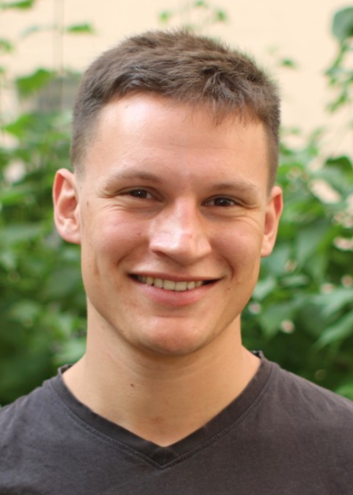
\includegraphics[width=\textwidth]{img/paul.png}\hspace{1em}
\end{minipage}
\hfill
\begin{minipage}[t]{1\textwidth}
    \vspace{0pt}
    \begin{shaded*}
        \begin{minipage}[t]{0.47\textwidth}
            \vspace{0pt}
            {\par\centering\huge{Paul Brenker}} \\[0.3cm]
            \faGlobe~ Nationality: German\\
            \faBirthdayCake~ 1996 \\
            \faMapMarker~ Berlin, Germany \\
            \begin{spacing}{0.5}
                {
                    \faCommentsO~ \underline{Languages:} \\
                    \begin{tabular}{l l}
                        \emph{German:} native & \emph{English:} full working proficiency \\
                        \emph{Hebrew:} intermediate proficiency & \emph{Arabic:} basic knowledge \\ 
                    \end{tabular}
                }
            \end{spacing}
            \vspace{4pt}
        \end{minipage}\hfill
        \begin{minipage}[t]{0.36\textwidth}
            \vspace{29pt} 
            \faPhone~ +972 52 3002843 \\
            \faPhone~ +49 173 5287524 \\

            \faAt~ \protect\url{paul.brenker@gmail.com} \\
           % \faEnvelopeO~ Maxstr. 28, 53111 Bonn \\
            \faGithub~ \protect\url{github.com/paulbrenker} \\
            \faLinkedin~ \protect\url{linkedin.com/in/paul-brenker}\\
        \end{minipage}
        \hfill
    \end{shaded*}
\end{minipage}\\[15pt]
\subsection*{}
\vspace{-3em}
\setlength{\columnsep}{1.7cm}
\columnratio{0.47}[0.46]
\begin{paracol}{2}
    \hbadness5000
    \paracolbackgroundoptions
    %\small
    \section*{Experience}
    \begin{minipage}[t]{\leftcolwidth}
        \begin{tabular}{p{0.18\textwidth}| p{0.65\textwidth}}
            \cvevent{2023 - 2024}{SAP LeanIX}{Working Student}{Bonn, Germany}{Contributed to the LeanIX EAM product as part of an agile engineering team. Learned to work with numerous technologies used in microservice architectures. Developed Backend REST Endpoints of the new Documents feature in LeanIX EAM. Established internal best practices for dealing with cursor based pagination in combination with dynamical filtering using the Java Persistence API.}{img/leanix_logo.jpg}\\
            \cvevent{2023}{LeanIX}{Intern}{Bonn, Germany}{Investigated and implemented evaluation tools for OpenAPI specifications. Developed a prototype for company-wide integration pipeline using GitHub Actions}{img/leanix_logo_old.jpg}\\
            \cvevent{2022 - 2023}{University of Bonn}{Student assistant}{Bonn, Germany}{Administration and maintenance of institute for philosophy websites and IT equipment.}{img/uni_bonn_logo.png}\\
            \cvevent{2017 - 2018}{Academy of Sciences and Humanities}{Student Assistant}{Berlin, Germany}{Transcription of ancient Hebrew and Arabic texts. XML annotation of academic text for cross-referenced usage in a database. Proofreading of articles.}{img/bbaw_logo.jpg}
        \end{tabular}
        \bigskip
        \begin{minipage}[t]{\leftcolwidth}
            \section*{Skills}
            {\normalsize
            \begin{tabular}{l l l}
                \textbf{Programming} & \textbf{Frameworks} & \textbf{Other} \\
                \emph{Java} & \emph{Spring Boot} & Functional Programming\\
                \emph{Kotlin} & \emph{Java Persistence API} & Agile Methodologies \\
                \emph{NodeJS} & \emph{Angular} & \emph{REST APIs} \\
                \emph{Python} & GitHub Actions & CI/CD Pipelines \\
                LaTeX & PostgreSQL & Databases \\
                & & Git, Linux, Docker \\
                & & Data Analysis \& Visualization \\ 
                & & Machine learning \\
            \end{tabular}
            }
        \end{minipage}\hfill
    \end{minipage}
    \switchcolumn
    \begin{minipage}[t]{\rightcolwidth}
        \section*{Education}
        \begin{tabular}{p{0.18\textwidth}| p{0.65\textwidth}}
            \cvevent{2019 - 2024}{Bonn-Rhein-Sieg University of Applied Sciences (H-BRS)}{B.S. Computer Science}{Bonn, Germany}{Computer Science degree with a final grade of 1.6 GPA (90 \%) within the best 10 \% of faculty graduates. Specialized in Bioinformatics and Data Science where I did multiple applied projects. For my Thesis I chose the topic: Relevance of OpenAPI Linter Rules for Specification Quality.}{img/hbrs_logo.jpg} \\
            \cvevent{2015 - 2019}{Freie Universität zu Berlin}{B.A. History and Culture of the Middle East}{Berlin, Germany}{Language centered degree with long time abroad language courses in Egypt, Israel and Jordan. Thesis was written about gender-specific variations in the Arabic dialect of Amman, Jordan}{img/fu_logo.png} \\
        \end{tabular}
    \bigskip
    \begin{minipage}[t]{\rightcolwidth}
        \section*{Scholarships}
        \begin{tabular}{>{\bfseries}p{0.12\textwidth} >{}p{0.7\textwidth}}
            2023 & Deutschlandstipendium -  Scholarship for ambitious and talented students                                                  \\
            2018 & Scholarship for a full Semester of intensive Arabic language courses at the German Jordanian University in Amman, Jordan. \\
            2018 & PROMOS -  Scholarship for an intensive Hebrew summer school at the Ben Gurion University of the Negev                     \\
        \end{tabular}
    \end{minipage}\hfill
    \bigskip
    \begin{minipage}[t]{\rightcolwidth}
        \section*{Volunteering}
        \begin{tabular}{>{\bfseries}p{0.12\textwidth} >{}p{0.7\textwidth}}
            2014 & After graduating from high school I volunteered for nine months in Kibbutz Ein Hashlosha in Israel. During my time I worked mostly in agriculture and landscaping but also in the local garage where I helped to maintain the vehicles of the Kibbutz. \\
        \end{tabular}
        \bigskip
        \section*{Hobbies}
        \begin{tabular}{>{\bfseries}p{0.12\textwidth} >{}p{0.7\textwidth}}
            Rowing  & I row since I am ten years old and participated in countless competitions including the German national sprint league. \\
            Cycling & I love to ride bicycles not just for sport but also in the everyday for a sustainable and balanced life.
        \end{tabular}
    \end{minipage}
\end{minipage}
\end{paracol}

%\vfill{} % Whitespace before final footer
%----------------------------------------------------------------------------------------
%	FINAL FOOTER
%----------------------------------------------------------------------------------------
% \setlength{\parindent}{0pt}
% \begin{minipage}[t]{\textwidth}
%     \begin{center}\fontfamily{\sfdefault}\selectfont \color{black!70}
%         {\small Paul Brenker 
%         %\icon{\faEnvelopeO}{black}{} Maxstr. 28 
%         \icon{\faMapMarker}{black}{} Tel Aviv 
%         \icon{\faPhone}{black}{} +972 52 3002843
%         \icon{\faPhone}{black}{} +49 173 5287524
%         \icon{\faAt}{black}{} \protect\url{paulbrenker@gmail.com}
%         }
%     \end{center}
% \end{minipage}
\end{document}